\chapter{Introduction}
\label{chapter1}

\section{Context}
Cloud computing has always been seen as a way of improving compute performance by the use of multiple computers connected to each other. The games industry has rapidly evolved along the years and a great deal of demand is apparent. Developers of games have pushed computer hardware to meet the needs of consumers for more complicated games and realism. Even with computer hardware becoming cheaper and more of a commodity, the costs of driving graphics rendering for high-end games to run at the optimal settings of 1080p at 60fps are still relatively high.

\section{Project Aim}
The aim of the project is to produce a solution which uses software-defined networking to reduce the network latency in a network in terms of a cloud gaming system.

\section{Project Objectives}
\begin{itemize}
  \item A simple game program, that is computationally expensive enough to not perform optimally on a single machine (simple flight simulator with real time procedurally generated trees).
  \item A simplified cloud gaming system where the game created is launched on the cloud and input on the client side in the form of button presses on the keyboard is sent to the game on the server. The game frames produced are then sent to the client's screen.
  \item Produce a virtual network with simulated cloud game traffic and delay. With the use of SDN, reduce latency in the network.
\end{itemize}

\section{Deliverables}
The deliverables of the project include:
\begin{itemize}
  \item Code that demonstrates a simple game/simulation rendering graphics on a server and controlled by a client remotelyand a manual on how to setup the client and server for the cloud gaming system.
  \item Code that creates a virtual network and software-defined networking load balancer as well as a manual on how to set it up and run the code and softtware.
  \item Project report that explains the problem the project is trying to solve and the schematics of the solution produced as well as an evaluation of the solution.
\end{itemize}

\section{Methodology}

\subsection{Project Schedule}
\begin{figure}[h]
 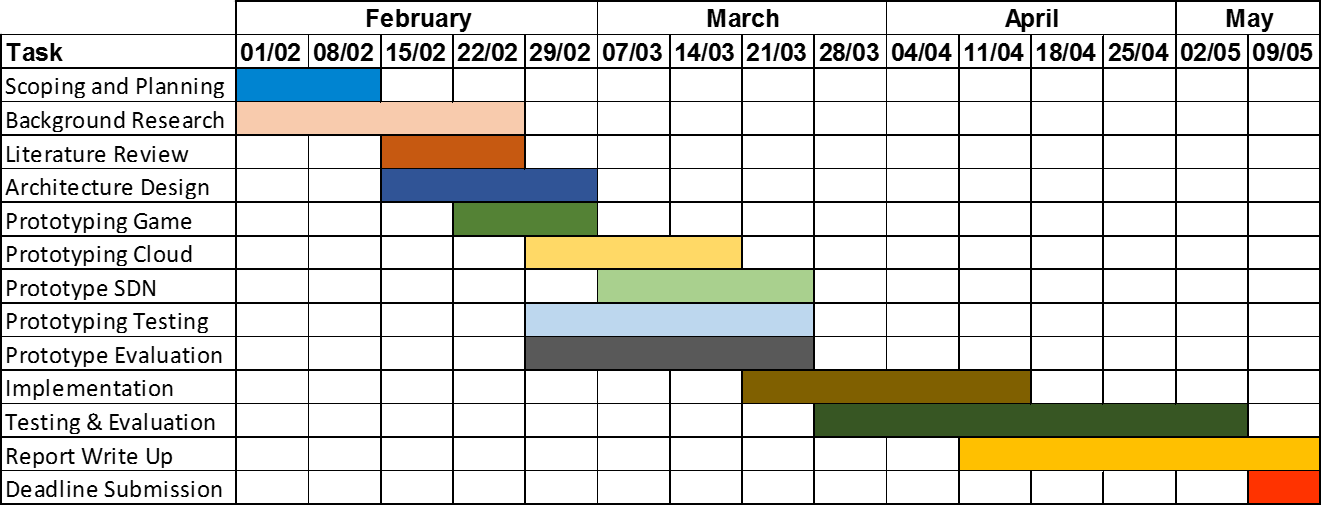
\includegraphics[width=\linewidth]{images/gantt.png}
 \caption{Gantt chart of project schedule}
 \label{fig:schedule}
\end{figure}

\subsection{Methodology}
The approach that was used for this project was iterative. Iterative process means doing an initial plan followed by an iteration of planning, design, implementation, testing then evaluation. This iteration is repeated again to improve the prototype. An iteration of the project development is outlined below.
\newline
\par
The problem and scope of the project was first defined and this includes background research After doing background research, the next process was literature review of the information I have found. Comparisons of different techniques that reduce or mask latency and increase the overall performance of the system was made. A single technique was then chosen to focus on and this was software-defined networking. The next step was to design the architecture for the cloud gaming system along with how it will be implemented:
\newline
\par
A prototype of the game was produced and was made sure it was running properly on a single system in the DEC-10 Lab. The game rendered a procedurally generated tree using Lindenmayer system which is computationally expensive to produce in real time. The game also uses lighting and shadows which adds more to the compute power needed. The game area can be navigated around by the player using simple flight simulator controls.
\newline
\par
When this was completed, a server-client system where the server can receive user input from a client and relay the commands to the OpenGL program was prototyped. The intention of this was to stream the rendered frames in video format to the client's window and the bandwidth of the video traffic was to be recorded. Simulated traffic was then used on a virtual network for the SDN solution which was tested against different test scenarios and evaluated.

\subsection{Version Control}
The project uses version control for both the code development and report write up. A public GitHub repository was created and development changes were saved as the project progressed. This is so backups are created regularly just in case some new code broke the implementation, an older version can be easily loaded back up. The code repository is also hosted remotely so it can be accessed using multiple machines and not in one machine. This protect against losing files accidentally if it was stored locally. The GitHub public repository is hosted using the following link:
\url{http://github.com/kvcruzat/cloudgaming/}.